\section{Machine Learning Models}
\label{sec:ML_Models}
\subsection{Introduction}
In this section, we present and discuss the machine learning models implemented in this project, focusing on their structure, functionality, and contributions to the energy consumption prediction problem. These models fall within the supervised learning paradigm for regression tasks and are specifically designed to address the challenges of forecasting energy consumption patterns.

We begin with an in-depth exploration of several model architectures, including Random Forest, Feedforward Neural Networks (FNNs), and Recurrent Neural Networks (RNNs) with Long Short-Term Memory (LSTM) cells. Each model leverages unique mechanisms to process and learn from the data, enabling accurate prediction of energy consumption values. Furthermore, we describe the hyperparameter tuning strategies employed to optimize these models for enhanced performance, as well as data preprocessing techniques used to improve model generalization.

Finally, we outline the evaluation metrics used to assess the models' effectiveness. These metrics provide a comprehensive understanding of the models' predictive accuracy, robustness, and suitability for the energy consumption regression task.


\subsection{Random Forest}
Random Forest is an ensemble learning method that operates by constructing multiple decision trees during training and outputting the mean prediction of the individual trees for regression tasks. This approach combines the predictions from many decision trees to reduce overfitting and improve accuracy.

\begin{figure}[h!]
    \centering
    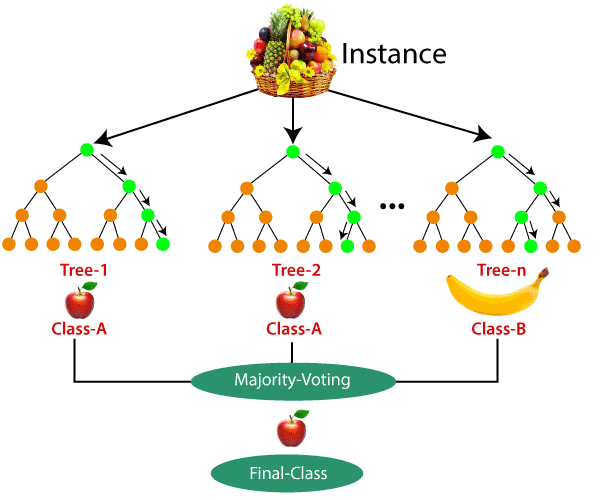
\includegraphics[width=0.8\linewidth]{images/rf_struture.png}
    \caption{Structure of a Random Forest}
    \label{fig:feedforward_structure}
\end{figure}

The algorithm works by creating multiple decision trees, each trained on a random subset of the data and features. For a Random Forest with N trees, the mathematical representation of the final prediction is:

\[
\hat{y} = \frac{1}{N}\sum_{i=1}^{N} f_i(x)
\]
where:
\begin{itemize} 
    \item $\hat{y}$ is the predicted energy consumption value
    \item $f_i(x)$ is the prediction of the i decision tree
    \item $N$ is the total number of trees in the forest
\end{itemize}

Random Forest offers several advantages for energy consumption prediction:

\begin{enumerate}
    \item Feature Importance: It provides insights into which features (e.g., time of day, weather conditions, historical consumption patterns) most significantly impact energy consumption.
    \item Robustness to Outliers: The ensemble nature of Random Forest makes it less sensitive to outliers in the training data.
    \item Handling Non-linearity: It can capture complex non-linear relationships between features and energy consumption without requiring feature transformation.
    \item Reduced Overfitting: By aggregating predictions from multiple trees, Random Forest reduces the risk of overfitting compared to individual decision trees.
\end{enumerate}

The hyperparameters tuned for our Random Forest model include:

\begin{itemize}
    \item Number of trees (n\_estimators)
    \item Maximum depth of trees (max\_depth)
    \item Minimum samples required to split a node (min\_samples\_split)
    \item Minimum samples required at a leaf node (min\_samples\_leaf)
\end{itemize}

\subsection{Feedforward Neural Networks (FNN)}

A Feedforward Neural Network (FNN) is designed to approximate complex functions by mapping input data to output values through a series of hidden layers. For our energy consumption prediction task, the FNN processes information in one direction from the input layer, through the hidden layers, to the output layer without forming cycles or loops.

\begin{figure}[h!]
    \centering
    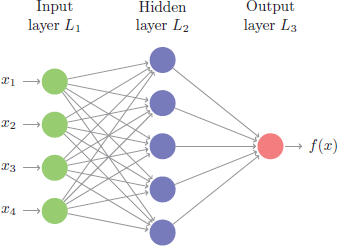
\includegraphics[width=0.8\linewidth]{images/fnn-struture.png}
    \caption{Structure of Feedforward Neural Networks (FNN)}
    \label{fig:feedforward_structure}
\end{figure}

Each neuron in an FNN is a computational unit that applies a weighted sum of its inputs, adds a bias, and passes the result through an activation function. Mathematically, this process can be expressed as:

\[
    y = f(\sum_{i=1}^{N} w_ix_i + b)
\]

where:

\begin{itemize}
    \item $y$ is the neuron's output
    \item $x_i$ are the inputs (features related to energy consumption)
    \item $w_i$ are the weights associated with the inputs
    \item $b$ is the bias term
    \item $f$ is the activation function (e.g., ReLU, Tanh, or Linear)
\end{itemize}

Our FNN architecture consists of three main types of layers:

\begin{enumerate}
    \item Input Layer: This layer receives the input data representing features like historical consumption, weather variables, and other relevant factors.
    \item Hidden Layers: These layers perform the bulk of the computation in the network. Each hidden layer applies a transformation to the data using weights, biases, and activation functions.
    \item Output Layer: This layer produces the network's prediction, which is a single value representing the forecasted energy consumption. For our regression task, the output layer uses a linear activation function.
\end{enumerate}

The training process of our FNN involves:

\begin{itemize}
    \item Forward Propagation: The input data passes through the network layer by layer, with each layer performing its computation.
    \item Loss Calculation: The difference between predicted energy consumption and actual values is measured using Mean Squared Error (MSE).
    \item Backpropagation: The gradient of the loss function with respect to each weight and bias is computed and propagated backward through the network.
    \item Optimization: Adam algorithm updates the weights and biases to minimize the loss, improving the network's predictions.
\end{itemize}

FNNs are well-suited for energy prediction tasks where the relationship between inputs and outputs may be complex and non-linear, but they require careful tuning to avoid overfitting.

\subsection{Long Short-Term Memory (LSTM)}
LSTMs are an extension of recurrent neural networks (RNNs) mainly introduced to handle situations where RNNs fail \cite{g4g_lstm}. These special networks are good at understanding sequences of data - sentences, time series, or music - where the order of inputs matter and predicting the next time step regarding the context of the input. 

The network uses a concept of memory much like the human brain does. For example to fully understand a sentence the brain needs to remember the earlier words to make sense of the next ones.
LSTM networks use a concept of memory through LSTM cells, which are the main difference that distinguish them from RNN networks and are represented in the image \ref{fig:lstm_cell}.

A cell decides what to keep remembering, what to forget, what new information to learn, and what to output. These tasks are handled by three gates: the forget, the input, and the output gates. The forget gate decides what to forget from memory, the input gate decides what new information to add to memory, and the output gate decides what to pass on to the next step. All of these gates in a single cell work together to let the LSTM keep track of relevant information over time, even if the relevant information happened many steps ago.

\begin{figure}[h!]
    \centering
    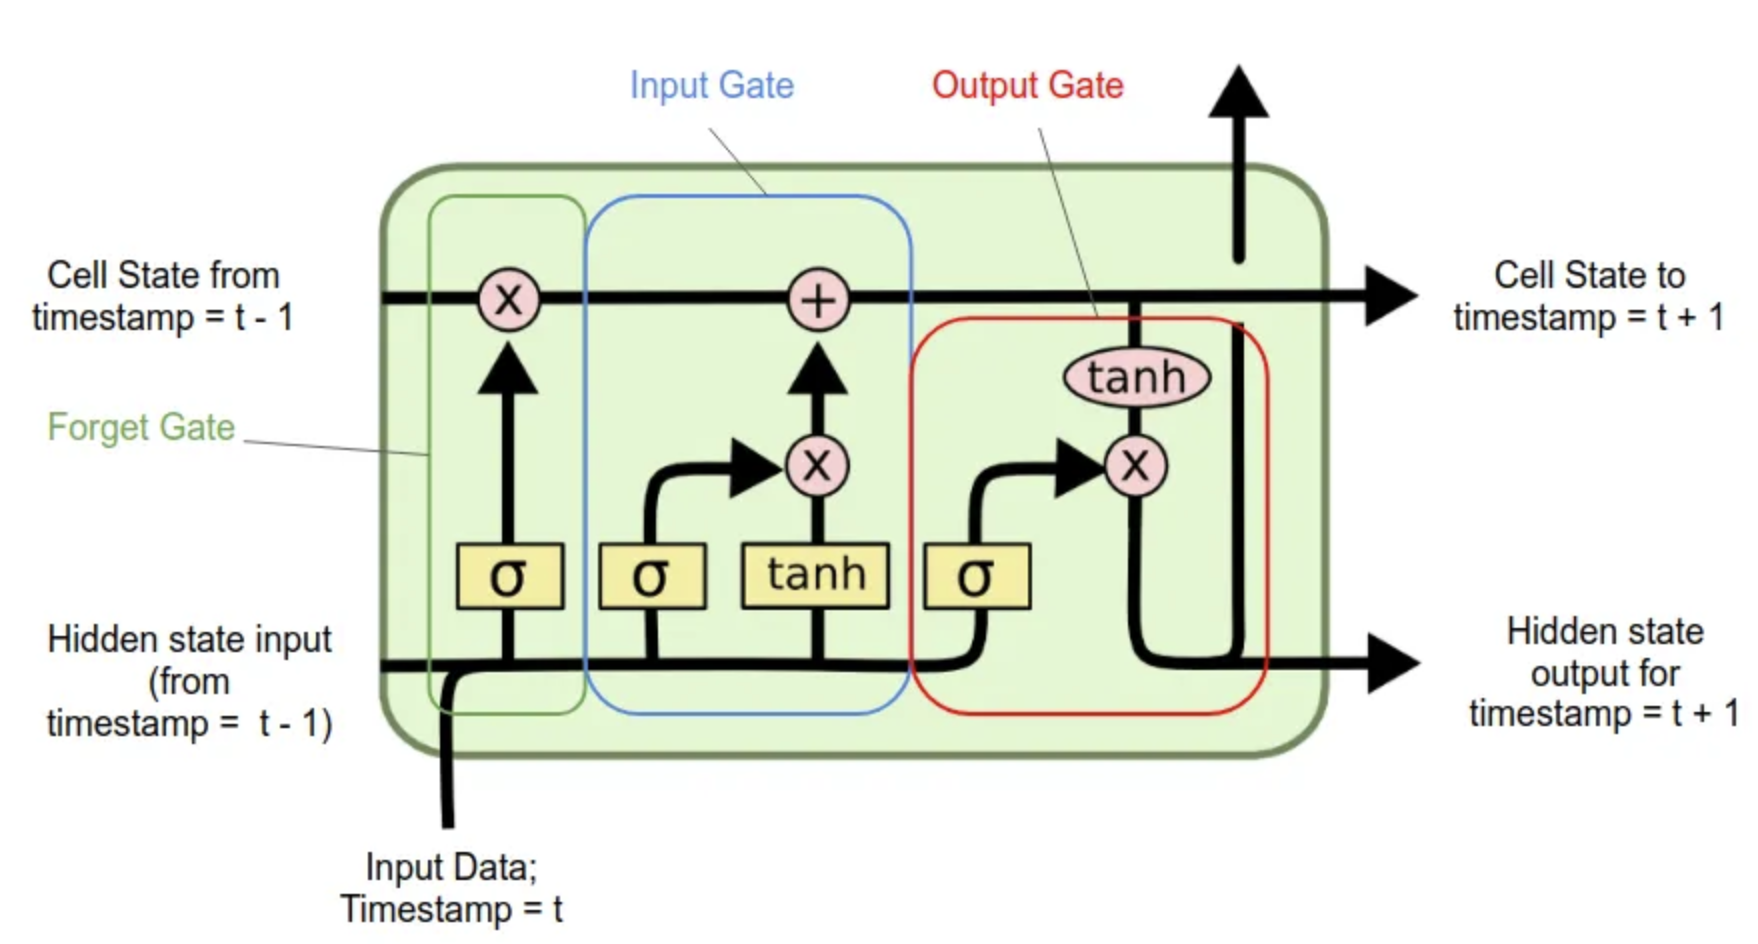
\includegraphics[width=0.8\linewidth]{images/lstm_cell.png}
    \caption{A single LSTM Cell \cite{medium_lstm}.}
    \label{fig:lstm_cell}
\end{figure}

In addition to the gates a single LSTM cell contains the "Cell state" and the "Hidden state". The Cell state encodes a kind of aggregation of data from all previous time steps that have been processed - it can be perceived as the memory of the cell while the Hidden state encodes the data from the most recent time step that has been processed. The Hidden state is not the output (or prediction) but merely an encoding that can be processed to obtain meaningful data.

Each of the gates follows this general equation:
\[f_t = \sigma((W_{hf}\times h_{t-1}) + (W_{xf} \times x) + b_f)\]
The inputs of these equations are \(h_{t-1}\) - a copy of the hidden state from the previous time step, and \(x\) - a copy of the data input at the current time step. The tanh function at the input gate takes another copy of both the hidden state from the previous time step and the data input at the current time step and normalizes it between -1 and 1, instead of 0 and 1 which happens when the sigmoid is applied. 

With each gate's output there is some sort of point-wise or element-wise multiplication which results in a matrix of weights that are between 0 and 1. An example would be that if the forget gate outputs a matrix of values that are all close to 1, it means the forget gate has concluded that based on the current input, the time-series' history is very important, and therefore, when the cell state from the previous time-step is multiplied by the forget gate's output, the cell state continues to retain most of its original value - "remember its past". If the forget gate outputs a matrix of values that are all very close to 0 then the cell state's values are scaled down to small numbers which means the forget gate has told the network to forget most of its past up until the current time-step\cite{medium_lstm}.

\subsection{Data Preprocessing and Hyperparameter Tuning}

To enhance the performance and generalization of the machine learning models, this study employs two critical techniques: data Preprocessing and hyperparameter tuning.

\subsubsection{Data Preprocessing}

For our energy prediction task, proper data preprocessing is essential to improve model performance. The following techniques were applied:

\begin{itemize}
    \item Feature Scaling: All numerical features were standardized or normalized to ensure that no single feature dominates the learning process due to its scale.
    \item Lag Features: Historical energy consumption values at different time lags were incorporated as features to provide context about recent consumption patterns.
    \item Missing Value Handling: Rather than applying imputation methods, we opted for a strict filtering approach. Only buildings with complete time series (from the beginning to the end of the study period) were retained in the dataset. Buildings with gaps or missing values were completely excluded from the analysis, ensuring the integrity and reliability of the data used for training and testing.
    \item Logarithmic Transformation: We applied logarithmic transformation to variables that exhibited heavily skewed distributions. This technique helped normalize the distribution of these variables, reducing the impact of extreme values and improving model performance.
\end{itemize}


\subsubsection{Hyperparameter Tuning}

Hyperparameter tuning involves systematically optimizing the key parameters that govern the training process and architecture of the models. 

Tuning was conducted using techniques like random search to identify the optimal combination of hyperparameters that minimize the validation loss. Cross-validation was employed to ensure robust performance across different subsets of the data.

By integrating comprehensive data preprocessing and hyperparameter tuning into the training workflow, our implemented models are better equipped to handle the challenges of energy consumption prediction, improving accuracy and robustness in the forecasts.


\subsection{Model Evaluation: Regression Metrics}

The evaluation of our energy prediction models was carried out using several regression metrics that provide complementary insights into model performance. These metrics help assess the accuracy, precision, and reliability of our predictions.

\subsubsection{Mean Squared Error (MSE)}

MSE measures the average squared difference between predicted and actual energy consumption values. It gives higher weight to larger errors due to the squaring operation, making it particularly sensitive to outliers.

\[
    MSE = \frac{1}{N}\sum_{i=1}^{N}( y_i - \hat{y_i})^2
\]
where:

\begin{itemize}
    \item $y_i$ is the actual energy consumption
    \item $\hat{y}_i$ is the predicted energy consumption
    \item $n$ is the number of samples
\end{itemize}

\subsubsection{Mean Absolute Error (MAE)}

MAE calculates the average absolute difference between predicted and actual values. It provides an intuitive understanding of prediction error in the same units as the energy consumption being predicted.

\[
    MAE = \frac{1}{N}\sum_{i=1}^{N}|y_i - \hat{y_i}|
\]
where:

\begin{itemize}
    \item $y_i$ is the actual energy consumption
    \item $\hat{y}_i$ is the predicted energy consumption
    \item $n$ is the number of samples
\end{itemize}

\subsubsection{Root Mean Square Error (RMSE)}

RMSE is the square root of the Mean Squared Error, providing a measure of the average magnitude of errors in the same units as the energy consumption being predicted. This makes it particularly interpretable in practical contexts.

\[
    RMSE = \sqrt{\frac{1}{N}\sum_{i=1}^{N}( y_i - \hat{y_i})^2}
\]

\subsubsection{Coefficient of Determination (R²)}

R² indicates the proportion of variance in the dependent variable (energy consumption) that is predictable from the independent variables. It ranges from 0 to 1, with higher values indicating better fit.

\[
    R² =  1 -\frac{\sum_{i=1}^{N}( y_i - \hat{y_i})^2}{\sum_{i=1}^{N}( y_i - \bar{y_i})^2}
\]

This metric provides an intuitive measure of how well the model captures the variations in energy consumption patterns.


\subsubsection{Training Loss}
Training loss quantifies how well the model fits the training data by calculating the difference between predicted and actual values. It is computed using a loss function such as cross-entropy for classification or mean squared error for regression. A lower loss means better model predictions. The goal during training is to minimize loss, but low training loss doesn’t always imply good generalization—overfitting can occur if the model is too closely fit to the training data.

\subsubsection{Visual Evaluation}

In addition to numerical metrics, we created several visualization plots to provide insights into model performance:

\begin{itemize}
    \item Residuals vs Actual Energy Consumption: This plot displays the prediction errors (residuals) on the y-axis against the actual energy consumption values on the x-axis. The ideal pattern shows residuals randomly scattered around the zero line with consistent variance across all energy consumption levels.
    \item Distribution of Prediction Errors: This histogram visualizes the frequency distribution of prediction errors. In an ideal scenario, errors should be centered around zero (indicating unbiased predictions), follow an approximately normal distribution, have minimal spread (narrow distribution) and show few outliers. This plot helps assess whether errors are systematic or random and provides insight into the overall error characteristics. A skewed distribution might suggest that the model consistently over or underestimates energy consumption, while heavy tails indicate frequent large errors.
    \item Predicted vs Actual Energy Consumption: This scatter plot compares predicted energy consumption values (y-axis) against actual observed values (x-axis), with a 45-degree reference line representing perfect predictions. Points should ideally cluster tightly around this line.
    \item Learning Curves:  Plots showing the evolution of MSE, MAE, and R² across training epochs help monitor the training process and identify potential overfitting.
\end{itemize}

By combining these complementary metrics and visualizations, we can thoroughly assess the strengths and weaknesses of each model for energy consumption prediction. This comprehensive evaluation approach guides model selection and further refinement to achieve the most accurate and reliable energy forecasts.